\RequirePackage{fix-cm}
\documentclass[smallextended]{svjour3}       % onecolumn (second format)
\smartqed  % flush right qed marks, e.g. at end of proof
\usepackage{graphicx,multicol,lipsum,caption,authblk}
\usepackage{amsmath,booktabs,verbatim,tikz}
\usepackage{geometry,pgf,pgfplots,}
\usepackage{mathptmx}
\usetikzlibrary{shapes.geometric, matrix,arrows,positioning,calc,intersections}
\usepackage{booktabs, makecell, multirow, threeparttable}
\usepackage{tablefootnote}
\begin{document}



\title{Laminated Composite Plate Optimization by Genetic Algorithm}
\titlerunning{Stacking Sequence Optimization}        % if too long for running head
\author{Zhang Huiyao$^1$  \and
	Atsushi Yokoyama $^{1,*}$
}
\authorrunning{Zhang Huiyao} % if too long for running head
\institute{Zhang Huiyao \at
              Room 203,Bulding 3,Kyoto Institue of Technology\\
			  Matsugasaki,Sakyo-ku,Kyoto,606-8585,JAPAN\\
              \email{zhanghy1012@gmail.com}           %  \\
           \and
           S. Author \at
              second address
}
\date{Received: date / Accepted: date}
\maketitle

\begin{abstract}
Failure analysis of laminated composite plates under different mechanical loads for different
stacking sequences, fiber orientation, and composite material system is studied in this paper.
An optimum composite material and laminate layup is studied for a targeted strength ratio which
makes a compromise between weight and cost through genetic algorithm.


\keywords{Genetic Algorithm \and Laminates \and Stacking Sequence \and Hybrid Composites}
\end{abstract}

%\begin{multicols}{2}
%\begin{multicols}


\section{Introduction}
% 第一段
% 第一句话,FRP复合材料在众多领域都有着广泛的应用,因为它具有很高的强度比等性质.
Composites material offer improved strength, stiffness, fatigue, and corrosion resistance, etc over
conventional materials, which is widely used in automotive, aerospace, and ship building industry.
However, the high cost of fabrication of composites is a critical drawback for its application, for
example, the graphite/epoxy composite part may cost as much as \$650 to \$900 per kilogram.
The mechanical performance of a composite is affected by a wide range of factors, fiber length,
fiber orientation, fiber shape, and the matrix etc.




% 第三句话,各种关于这种材料的优化都使用遗传算法

% 第二段
% 第一句介绍遗传算法
Genetic algorithms(GAs) simulate the process of natural evolutionary includes selection, crossover ,and mutation  according to Darwin's principal of "survival of the fittest".
% 第二句 列出最近几个遗传算法的应用

According to T Back \cite{back1994selective},the selection mechanism is one of the primary means of controlling the GA's convergence rate and its
likelihood of finding global optima.




\section{Stress and Strain in a Laminate}
A laminated structure is consisting of multiple laminas bonded together through their thickness.
Consider a laminated composite plate which is symmetric to its middle plane and subjected to in-plane
loads of extension, shear, bending and torsion,  the classical lamination theory(CLT) is taken to
calculate the stresses and strains in the local and global axes of each ply. as shown in
Fig.\ref{fig:lamina}.

\begin{center}
  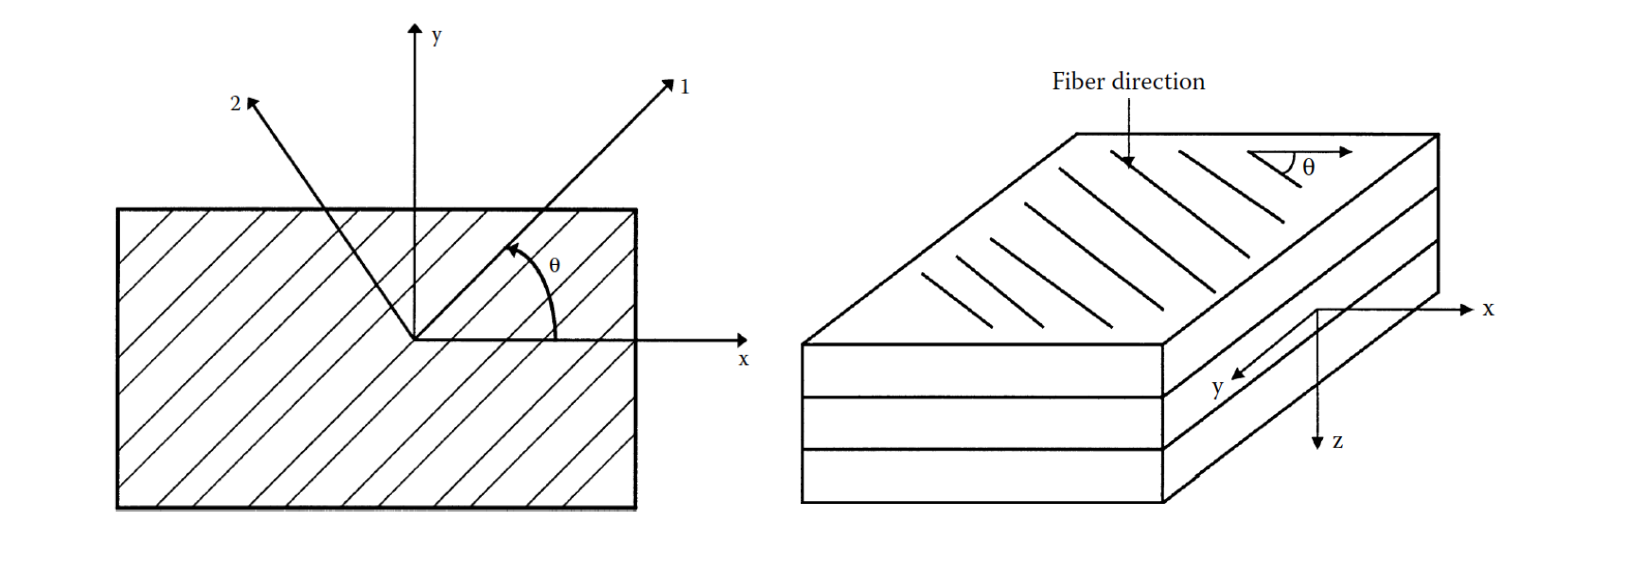
\includegraphics[width=\linewidth]{A_laminate_design_images/lamina_local_global_axes.png}
  \captionof{figure}{Lamina}
  \label{fig:lamina}
\end{center}

\subsection{Stress and Strian in a Lamina}
For a single lamina, the stress strain relation in the local axis.
\begin{equation}
    \begin{bmatrix}
        \sigma_1\\
        \sigma_2\\
        \tau_{12}
    \end{bmatrix}
    =
    \begin{bmatrix}
        Q_{11} & Q_{12} & 0\\
        Q_{12} & Q_{22} & 0\\
        0      &  0     & Q_{66}
    \end{bmatrix}
    \begin{bmatrix}
        \varepsilon_1\\
        \varepsilon_2\\
		\gamma_{12}
    \end{bmatrix}
\end{equation}
Where $Q_{ij}$ are the stiffnesses of the lamina that are related to 
engineering elastic constants by
\begin{equation}
    \begin{split}
    &Q_{11}=\frac{E_1}{1-v_{12}v_{21}}\\
    &Q_{22}=\frac{E_2}{1-v_{12}v_{21}}\\
    &Q_{66}=G_{12}\\
    &Q_{12}=\frac{v_{21}E_2}{1-v_{12}v_{21}}\\
    \end{split}
\end{equation}

Where, $E_1, E_2, v_{12}, G_{12}$ are four independent engineering elastic constants, they are
defined as 
\vspace{3mm}

$E_1$ = longitudinal Young's modulus(in direction 1)

$E_2$ = transverse  Young's modulus(in direction 1)

$v_{12}$ = major Poisson's ratio

$G_{12}$ = in-plane shear modulus (in plane 1-2)
\vspace{3mm}

Stress strain relation in global axis are

\begin{equation}
	\left[\begin{array}{l}\sigma_{x} \\ \sigma_{y} \\ \tau_{x
			y}\end{array}\right]=\left[\begin{array}{lll}\bar{Q}_{11} & \bar{Q}_{12} & \bar{Q}_{16}
			\\ \bar{Q}_{12} & \bar{Q}_{22} & \bar{Q}_{26} \\ \bar{Q}_{16} & \bar{Q}_{26} &
			\bar{Q}_{66}\end{array}\right]\left[\begin{array}{l}\varepsilon_{x} \\ \varepsilon_{y}
	\\ \gamma_{x y}\end{array}\right]
\end{equation}

where

\begin{equation}
	\begin{array}{l}
		\bar{Q}_{11}=Q_{11} c^{4}+Q_{22} s^{4}+2\left(Q_{12}+2 Q_{66}\right) s^{2} c^{2}
		\\ 
		\bar{Q}_{12}=\left(Q_{11}+Q_{22}-4 Q_{66}\right) s^{2} c^{2}+Q_{12}\left(c^{4}+s^{2}\right)
		\\ 
		\bar{Q}_{22}=Q_{11} s^{4}+Q_{22} c^{4}+2\left(Q_{12}+2 Q_{66}\right) s^{2} c^{2} \\

		\bar{Q}_{16}=\left(Q_{11}-Q_{12}-2 Q_{66}\right) c^{3} s-\left(Q_{22}-Q_{12}-2
			Q_{66}\right) s^{3} c \\ 
		\bar{Q}_{26}=\left(Q_{11}-Q_{12}-2 Q_{66}\right) c s^{3}-\left(Q_{22}-Q_{12}-2 Q_{66}\right)
		c^{3} s \\ 
		\bar{Q}_{66}=\left(Q_{11}+Q_{22}-2 Q_{12}-2 Q_{66}\right) s^{2}
		c^{2}+Q_{66}\left(s^{4}+c^{4}\right)
	\end{array}
\end{equation}


The local and global stresses in an angle lamina are related to each other through the angle of
lamina $\theta$
\begin{equation}
	\left[\begin{array}{l}\sigma_{1} \\ \sigma_{2} \\ \tau_{12
			}\end{array}\right]=[T]\left[\begin{array}{l}\sigma_{x} \\ \sigma_{y} \\
	\tau_{xy}\end{array}\right]
\end{equation}

where 

\begin{equation}
	[T]=\left[\begin{array}{ccc}c^{2} & s^{2} & 2 s c \\ s^{2} & c^{2} & -2 s c \\ -s c & s c &
	c^{2}-s^{2}\end{array}\right]
\end{equation}

\subsection{Stress and Strain in a Laminate}


\begin{equation} \label{eq:force_and_moments}
	\begin{array}{l}

	\begin{bmatrix}
		N_x \\
		N_y \\
		N_{xy}
	\end{bmatrix}
	=
	\begin{bmatrix}
		A_{11} & A_{12} & A_{16} \\
		A_{12} & A_{22} & A_{26} \\
		A_{16} & A_{26} & A_{66} 
	\end{bmatrix}
    \begin{bmatrix}
		\varepsilon_x^0 \\
        \varepsilon_y^0 \\
		\gamma_{xy}^0
    \end{bmatrix} 
	+
	\begin{bmatrix}
		B_{11} & B_{12} & B_{16} \\
		B_{11} & B_{12} & B_{16} \\
		B_{16} & B_{26} & B_{66} 
	\end{bmatrix}
	\begin{bmatrix}
		k_x \\
		k_y \\
		k_{xy} 
	\end{bmatrix}  \\
	\\

	\begin{bmatrix}
		M_x \\
		M_y \\
		M_{xy}
	\end{bmatrix}
	=
	\begin{bmatrix}
		B_{11} & B_{12} & B_{16} \\
		B_{12} & B_{22} & B_{26} \\
		B_{16} & B_{26} & B_{66} 
	\end{bmatrix}
    \begin{bmatrix}
		\varepsilon_x^0 \\
        \varepsilon_y^0 \\
		\gamma_{xy}^0
    \end{bmatrix} 
	+
	\begin{bmatrix}
		D_{11} & D_{12} & D_{16} \\
		D_{11} & D_{12} & D_{16} \\
		D_{16} & D_{26} & D_{66} 
	\end{bmatrix}
	\begin{bmatrix}
		k_x \\
		k_y \\
		k_{xy} 
	\end{bmatrix}
	\end{array}
\end{equation}



where

\begin{equation}
    \begin{split}
    &A_{ij}
	=
	\sum_{k=1}^n(\overline{Q_{ij}})_k(h_k-h_{k-1}) \\
    &B_{ij}
	=
	\frac{1}{2}\sum_{k=1}^n(\overline{Q_{ij}})_k(h_k-h_{k-1}) \\
    &D_{ij}
	=
	\frac{1}{3}\sum_{k=1}^n(\overline{Q_{ij}})_k(h_k-h_{k-1}) \\
    \end{split}
\end{equation}

The $[A]$, $[B]$, and $[D]$ matrices are called the extensional, coupling, and bending stiffness
matrices.



\section{Failure Theories of an Angle Lamina}
\subsection{Failure Theories of an Angle Lamina}
Many different theories about the failure of an angle lamina have been developed for a
unidirectional lamina, such as maximum stress failure theory, maximum strain failure theory,
Tsai-Hill failure theory, and Tsai-Wu failure theory. The failure theories of a lamina are based on
the stresses in local axes in the material. There are four normal strength parameters and one shear
stress for a unidirectional lamina. The five strength parameters are

\vspace{3mm}

$(\sigma_1^T)_{ult}=$ Ultimate longitudinal tensile strength(in direction 1),

$(\sigma_1^C)_{ult}=$ Ultimate longitudinal compressive strength(in direction 1),

$(\sigma_2^T)_{ult}=$ Ultimate transverse tensile strength(in direction 2),

$(\sigma_2^C)_{ult}=$ Ultimate transverse compressive strength(in direction 2), and

$(\tau_{12})_{ult}=$ Ultimate in-plane shear strength

\vspace{3mm}

In this paper, Tsai-wu failure theory is taken to decide whether a lamina is failed or not, the
reason is chosen because this theory is  more general than Tsai-Hill failure theory which consider
two different situation, compressive and tensile strength of a lamina. A lamina is considered to be
failed if


\begin{equation} \label{eq:tsai_wu}
H_1 \sigma_1 + H_2 \sigma_2 + H_6 \tau_{12} + H_{11}\sigma_1^2 + H_{22} \sigma_2^2 + H_{66}
\tau_{12}^2 + 2H_{12}\sigma_1\sigma_2 < 1
\end{equation}
 
is violated. where


\begin{equation}
	\begin{array}{l}
		H_{1}=\frac{1}{\left(\sigma_{1}^{T}\right)_{u l t}}-\frac{1}{\left(\sigma_{1}^{C}\right)_{u l
	t}} \\
	H_{11}=\frac{1}{\left(\sigma_{1}^{T}\right)_{u l t}\left(\sigma_{1}^{C}\right)_{u l t}} \\
	H_{2}=\frac{1}{\left(\sigma_{2}^{T}\right)_{u l t}}-\frac{1}{\left(\sigma_{2}^{C}\right)_{u l
	t}} \\
	H_{22}=\frac{1}{\left(\sigma_{2}^{T}\right)_{u l t}\left(\sigma_{2}^{C}\right)_{u l t}} \\
	H_{66}=\frac{1}{\left(\tau_{12}\right)_{u l t}^{2}} \\
	H_{12}=-\frac{1}{2} \sqrt{\frac{1}{\left(\sigma_{1}^{T}\right)_{u l
				t}\left(\sigma_{1}^{C}\right)_{u l t}\left(\sigma_{2}^{T}\right)_{u l
	t}\left(\sigma_{2}^{C}\right)_{u l t}}}
	\end{array}
\end{equation}


The Equation \ref{eq:tsai_wu} can determin whether a lamina failed or not, but it failed to give the
information about how much load can be increased or decreased to keep the lamina safe. The strength
ratio(SR) is to used to solve this problem, and defined as

\begin{equation} \label{eq:sr}
	S R=\frac{\text {Maximum Load Which Can Be Applied}}{\text {Load Applied}}
\end{equation}


Substituting Equation \ref{eq:sr} for $SR$ into Equation \ref{eq:tsai_wu},we obtain
\begin{equation}
		(F_{11}\sigma_1^2+F_{22}\sigma_2^2+F_{66}\sigma_6^2+2F_{12}\sigma_1\sigma_2)SR^2 
						 +(F_1\sigma_1+F_2\sigma_2)SR-1=0
\end{equation}




\subsection{Failure Theories of a Laminate}

\begin{enumerate}
	\item Compute the reduced stiffness matrix $[Q]$ referred to local axis for each ply using its
		four engineering elastic constants $E_1$, $E_2$, $v_{12}$, and $G_{12}$.
	\item calculate the transformed reduced stiffness $[\bar{Q}]$ referred to global coordinate
		system (x, y) using reduced stiffness matrix $[Q]$ obtained in step 1 and ply angle for each layer.
	\item Given the thickness $t_k$ and the location of each layer, find out the three laminate
		stiffness matrices $[A]$, $[B]$, and $[D]$.
	\item Apply forces and moments, $[N]_{xy}$, $[M]_{xy}$, solve the equation
		\ref{eq:force_and_moments}, calculate the middle plane strain $[\sigma^0]_{xy}$ and
		cruvature $[k]_{xy}$.
	\item Find out the local strain and stress of each layer under the applied load.
	\item Use the ply-by-ply stresses and strains in Tsai-wu failure theory to find out the strenght
		ratio.
\end{enumerate}

\section {Genetic Algorithm Procedure}
\begin{center}
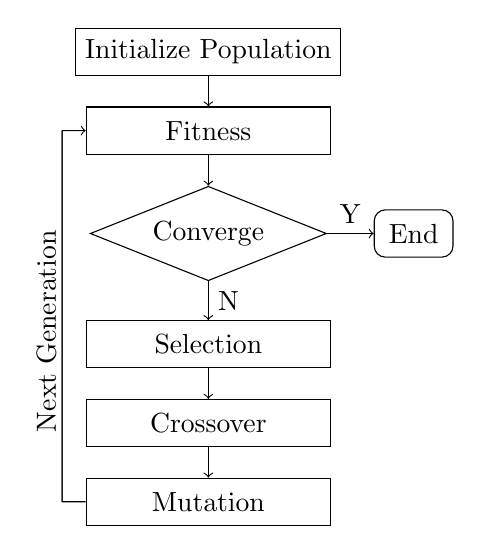
\begin{tikzpicture}
\tikzstyle{startstop} = [rectangle, rounded corners, minimum width=1.0cm,minimum height=0.6cm, 
                        text centered, draw=black]
\tikzstyle{io} = [trapezium, trapezium left angle=70, trapezium right angle=110, minimum width=2cm, 
                 minimum height=0.6cm, text centered, draw=black]
\tikzstyle{process} = [rectangle, minimum width=3.1cm, minimum height=0.6cm, text centered, draw=black]
\tikzstyle{decision} = [diamond,minimum width=3cm, minimum height=1.2cm, draw=black]
\node (population) [process] {Initialize Population};
\node (fitness) [process, below of=population] {Fitness};
\node (decision) [decision] at ($(fitness.south)+(0,-1.0cm)$) {} node at (decision.base) {Converge};
\node (share-fitness) at ($(decision.south)+(0,-0.8cm)$) [process] {Selection};
\node (selection) [process,below of=share-fitness] {Crossover};
\node (crossover) [process,below of=selection]  {Mutation};
\node (end) [startstop] at ($(decision.east)+(1.1cm,0)$)  {End};
\draw [->] (population) -- (fitness);
\draw [->] (fitness) -- (decision);
\draw [->] (decision) -- (share-fitness) node[auto=left,pos=0.5]{N};
\draw [->] (share-fitness.south) -- (selection.north) ;
\draw [->] (selection.south) -- (crossover.north);
\draw [->] (decision.east) -- (end.west) node[auto=left,pos=0.5]{Y};

% draw intersection
\draw [white] (fitness.west) -- ++(-0.5cm,0) coordinate (A);
\draw [white] (crossover.west) -- ++(-0.3cm,0) coordinate (B)-- ++(0,6cm) coordinate (C) ; 
\draw (crossover.west) -- ++(-0.3cm,0) -- (intersection cs: first line={(fitness.west)--(A)}, 
      second line={(B)--(C)}) coordinate (D);
\draw (B) -- (D) node[auto=left,pos=0.8,rotate=90,xshift=-0.2cm,yshift=0.2cm] {Next Generation} ;
\draw [<-] (fitness.west) -- (D);
\end{tikzpicture}
\captionof{figure}{GA Procedure with Share Function}
\label{plot:GA}
\end{center}


\section{Results and Discussion}

\captionof{table}{Typical Properties of a Unidirectional Lamina(SI System of Units)}
\begin{tabular}{ccccc}
	\toprule
	Property								  & Symbol	   & Unit &  Glass/Epoxy &  Graphite/Epoxy  \\
	\midrule
	Fiber volume fraction					  & $V_f$		      &      &  0.45        &  0.70   \\
	Longitudinal elastic modulus			  & $E_1$		      & GPa  &  38.6        &  181  \\
	Traverse elastic modulus				  & $E_2$		      & GPa  &  8.27        &  10.3  \\
	Major Poisson's ratio					  & $v_{12}$	      &      &  0.26        &  0.28  \\
	Shear modulus							  & $G_{12}$	      & GPa  &  4.14        &  7.17  \\
	Ultimate longitudinal tensile strength    &  $(\sigma_1^T)_{ult}$ & MPa  &  1062        &  1500  \\
	Ultimate longitudinal compressive strength & $(\sigma_1^C)_{ult}$ & MPa  &  610        &  1500  \\
	Ultimate transverse tensile strength    &  $(\sigma_2^T)_{ult}$ & MPa  &  31        &  40 \\
	Ultimate transverse compressive strength & $(\sigma_2^C)_{ult}$ & MPa  &  118        &  246\\
	Ultimate in-plane shear strength          & $(\tau_{12})_{ult}$ & MPa  &  72&  68\\
	\bottomrule
\end{tabular}


\captionof{table}{Comparative study of different composite materials for a defined strenght ratio}

\begin{tabular}{ccccccc}
	\toprule
	Load         &Type of composite & Stacking sequence    & Strength ratio  & Mass &  Cost   & Height\\
	\midrule
	           &Glass/Epoxy       & $[0]_{6s}$           & 2.103           & 0.707 &  12.0  & 1.980  \\
	$N_x=1e6$ N &Graphite/Epoxy    &  $[0]_9$             & 2.227           & 0.481 &  22.5  & 1.485 \\
	            &Hybrid composite  &  $[Gl${\text -}$E/Gr${\text -}$E_{5}]_s$ & 2.082  & 0.545 &  22.0  & 1.650 \\
	\bottomrule
\end{tabular}


\begin{tabular}{ccccccc}
	\toprule
	Load         &Type of composite & Stacking sequence    & Strength ratio  & Mass &  Cost   & Height\\
	\midrule
	           &Glass/Epoxy       & $[0]_{6s}$           & 2.103           & 0.707 &  12.0  & 1.980  \\
	$N_y=1e6$ N  &Graphite/Epoxy    &  $[0]_9$             & 2.227           & 0.481 &  22.5  & 1.485 \\
	            &Hybrid composite  &  $[Gl${\text -}$E/Gr${\text -}$E_{5}]_s$ & 2.082  & 0.545 &  22.0  & 1.650 \\
	\bottomrule
\end{tabular}


\begin{tabular}{ccccccc}
	\toprule
	Load         &Type of composite & Stacking sequence    & Strength ratio  & Mass &  Cost   & Height\\
	\midrule
	           &Glass/Epoxy       & $[0]_{6s}$           & 2.103           & 0.707 &  12.0  & 1.980  \\
	$N_{xy}=1e6$ N  &Graphite/Epoxy    &  $[0]_9$             & 2.227           & 0.481 &  22.5  & 1.485 \\
	            &Hybrid composite  &  $[Gl${\text -}$E/Gr${\text -}$E_{5}]_s$ & 2.082  & 0.545 &  22.0  & 1.650 \\
	\bottomrule
\end{tabular}


\begin{tabular}{ccccccc}
	\toprule
	Load         &Type of composite & Stacking sequence    & Strength ratio  & Mass &  Cost   & Height\\
	\midrule
	           &Glass/Epoxy       & $[0]_{6s}$           & 2.103           & 0.707 &  12.0  & 1.980  \\
	\makecell{$N_x=N_y=$ \\ $N_{xy}=1e6$ N}  &Graphite/Epoxy    &  $[0]_9$             & 2.227           & 0.481 &  22.5  & 1.485 \\
	            &Hybrid composite  &  $[Gl${\text -}$E/Gr${\text -}$E_{5}]_s$ & 2.082  & 0.545 &  22.0  & 1.650 \\
	\bottomrule
\end{tabular}

\captionof{table}{GA-parameters}
\begin{tabular}{cc}
	\toprule
	parameter & value \\
	\midrule
	population size      & 20               \\
    encoding method      & float encoding  \\
	selection strategy   & roulette wheel  \\
	crossover strategy   & one-point \\
	mutation strategy    & mass mutation   \\
	\bottomrule
\end{tabular}



\section{Concluding Remarks}
\section{Acknowledgements}
This is work was supported by 


%\end{multicols}
%\end{multicols}




The previous researchers adopted the first-ply-failure approach using the Tsai-wu failure
theory
\cite{massard1984computer,reddy1987first,fang1993design,soeiro1994multilevel,pelletier2006multi,jadhav2007parametric,omkar2008artificial}

minimize thickness
\cite{abu1998optimum,walker2003technique},weight\cite{fang1993design,deka2005multiobjective,park2008improved},
cost and weight\cite{deka2005multiobjective,omkar2008artificial}

Genetic Algorithm has been successfully applied to composite design
optimization\cite{riche1993optimization,nagendra1996improved,sadagopan1998application,todoroki1998stacking,liu2000permutation,sivakumar1998optimum,walker2003technique,lin2004stacking,kang2005minimum,murugan2007target,akbulut2008optimum}



\bibliographystyle{plain}
\bibliography{laminate_design}


\end{document}


